\documentclass{article}
\usepackage[utf8]{inputenc}
\usepackage[a4paper]{geometry}
\usepackage[T1]{fontenc}
\usepackage[brazil]{babel}
\usepackage[pdftex]{hyperref}
\usepackage{graphicx}
\graphicspath{ {/} }

\begin{document}
\begin{center}
{\LARGE \textsc{Universidade Estatual de Campinas}}\\[0.2cm]
{\LARGE \textsc{Instituto de Computação}}\\[3.5cm]
{\Large \textbf{Documentação do Projeto \\[0.2cm] Iniciação Científica}}\\[3.5cm]
{\large \textbf{Sistema Tutor Inteligente Mutimídia}}\\[4cm]
\end{center}

\begin{flushleft}
\textbf{Aluno:} André Figueiredo de Almeida \\
\textbf{Orientador:} Fábio Nauras Akhras \\
\textbf{Linha de Pesquisa:} Informática aplicada à educação
\vfill
\end{flushleft}

\begin{center}
Dezembro 2017
\end{center}
\pagenumbering{gobble}

\newpage
\pagenumbering{arabic}

\section{Sobre o projeto}
\subsection{Resumo}
Nesse trabalho foi desenvolvido um sistema computacional tutor inteligente, que aceita diferentes tipos de mídia. Ele foi desenvolvido de maneira a ser executado em um navegador de internet. Os conteúdos, compostos por diferentes tipos de mídia, questões e opções de resposta, são previamente definidos pelo educador e organizados em uma estrutura de grafo de forma a permitir múltiplos caminhos no ensino.

\subsection{Introdução}
Sistemas tutores inteligentes têm como objetivo auxiliar professores e alunos no processo educativo, usando modelos computacionais para automatizar e personalizar a sequência e/ou conteúdo apresentado ao estudante sobre algum tema [1]. O uso de mídias, como filmes, na educação tem sido estudado [2] de forma a abordar temas da sala de aula e discutir interpretações diferentes, além de estudos que combinam filmes com interação [3]. Somado a isso, estudos abordam estratégias construtivistas de educação em sistemas tutores [4], que é a metodologia que esse trabalho segue. Este trabalho teve como objetivo estudar esses conceitos teóricos e desenvolver um sistema tutor que tenha suporte para multimídia e que possibilite se adaptar ao aluno de acordo com suas respostas, além de ser leve e portátil para ser executado em máquinas com sistemas antigos/defasados.

\subsection{Discussão}

Para que o sistema tutor seja compatível com o maior número de máquinas possível, sem depender de instalação de softwares adicionais (que podem não ser compatíveis por motivos de hardware e/ou software), o sistema foi arquitetado para rodar em cima de um navegador de internet e foi escrito em HTML5, CSS e JavaScript. As funcionalidades do HTML5 tais como suporte a vídeo e áudio, e do CSS são suportadas pela maioria dos navegadores [5][6]. O código desenvolvido em JavaScript é compatível com 97\% dos navegadores atuais [7]. O HTML5 e o CSS são responsáveis pela interface gráfica (figura 1) e o JavaScript faz a parte computacional.

O educador deve, então, construir um conjunto de questões de múltipla escolha, associadas a conteúdos multimídia (vídeo, áudio, imagem). Ele deve então fazer uma relação entre as alternativas de resposta a cada questão (e conteúdo multimídia associado) e outras questões. A ideia é que, de acordo com a resposta do aluno, a questão seguinte tenha alguma relação com a resposta anterior, seguindo as teorias construtivistas [4]. Por exemplo, se o sistema tutor tem intenção de ensinar matemática, o educador pode criar respostas erradas que são geradas a partir de um erro de sinal na expressão. Na hora de construir a relação entre as respostas e outras questões, se o aluno optar por aquela resposta, o sistema leva a uma questão (e conteúdos multimídia associados) que reforça as regras de sinal. O sistema foi projetado de forma a ser genérico o suficiente para abordar inúmeras sequências, dando liberdade para vários cenários de adaptação. A responsabilidade da adaptabilidade fica, portanto, sobre a pessoa que projetar o sequenciamento de questões e conteúdos multimídia. 

\begin{center}
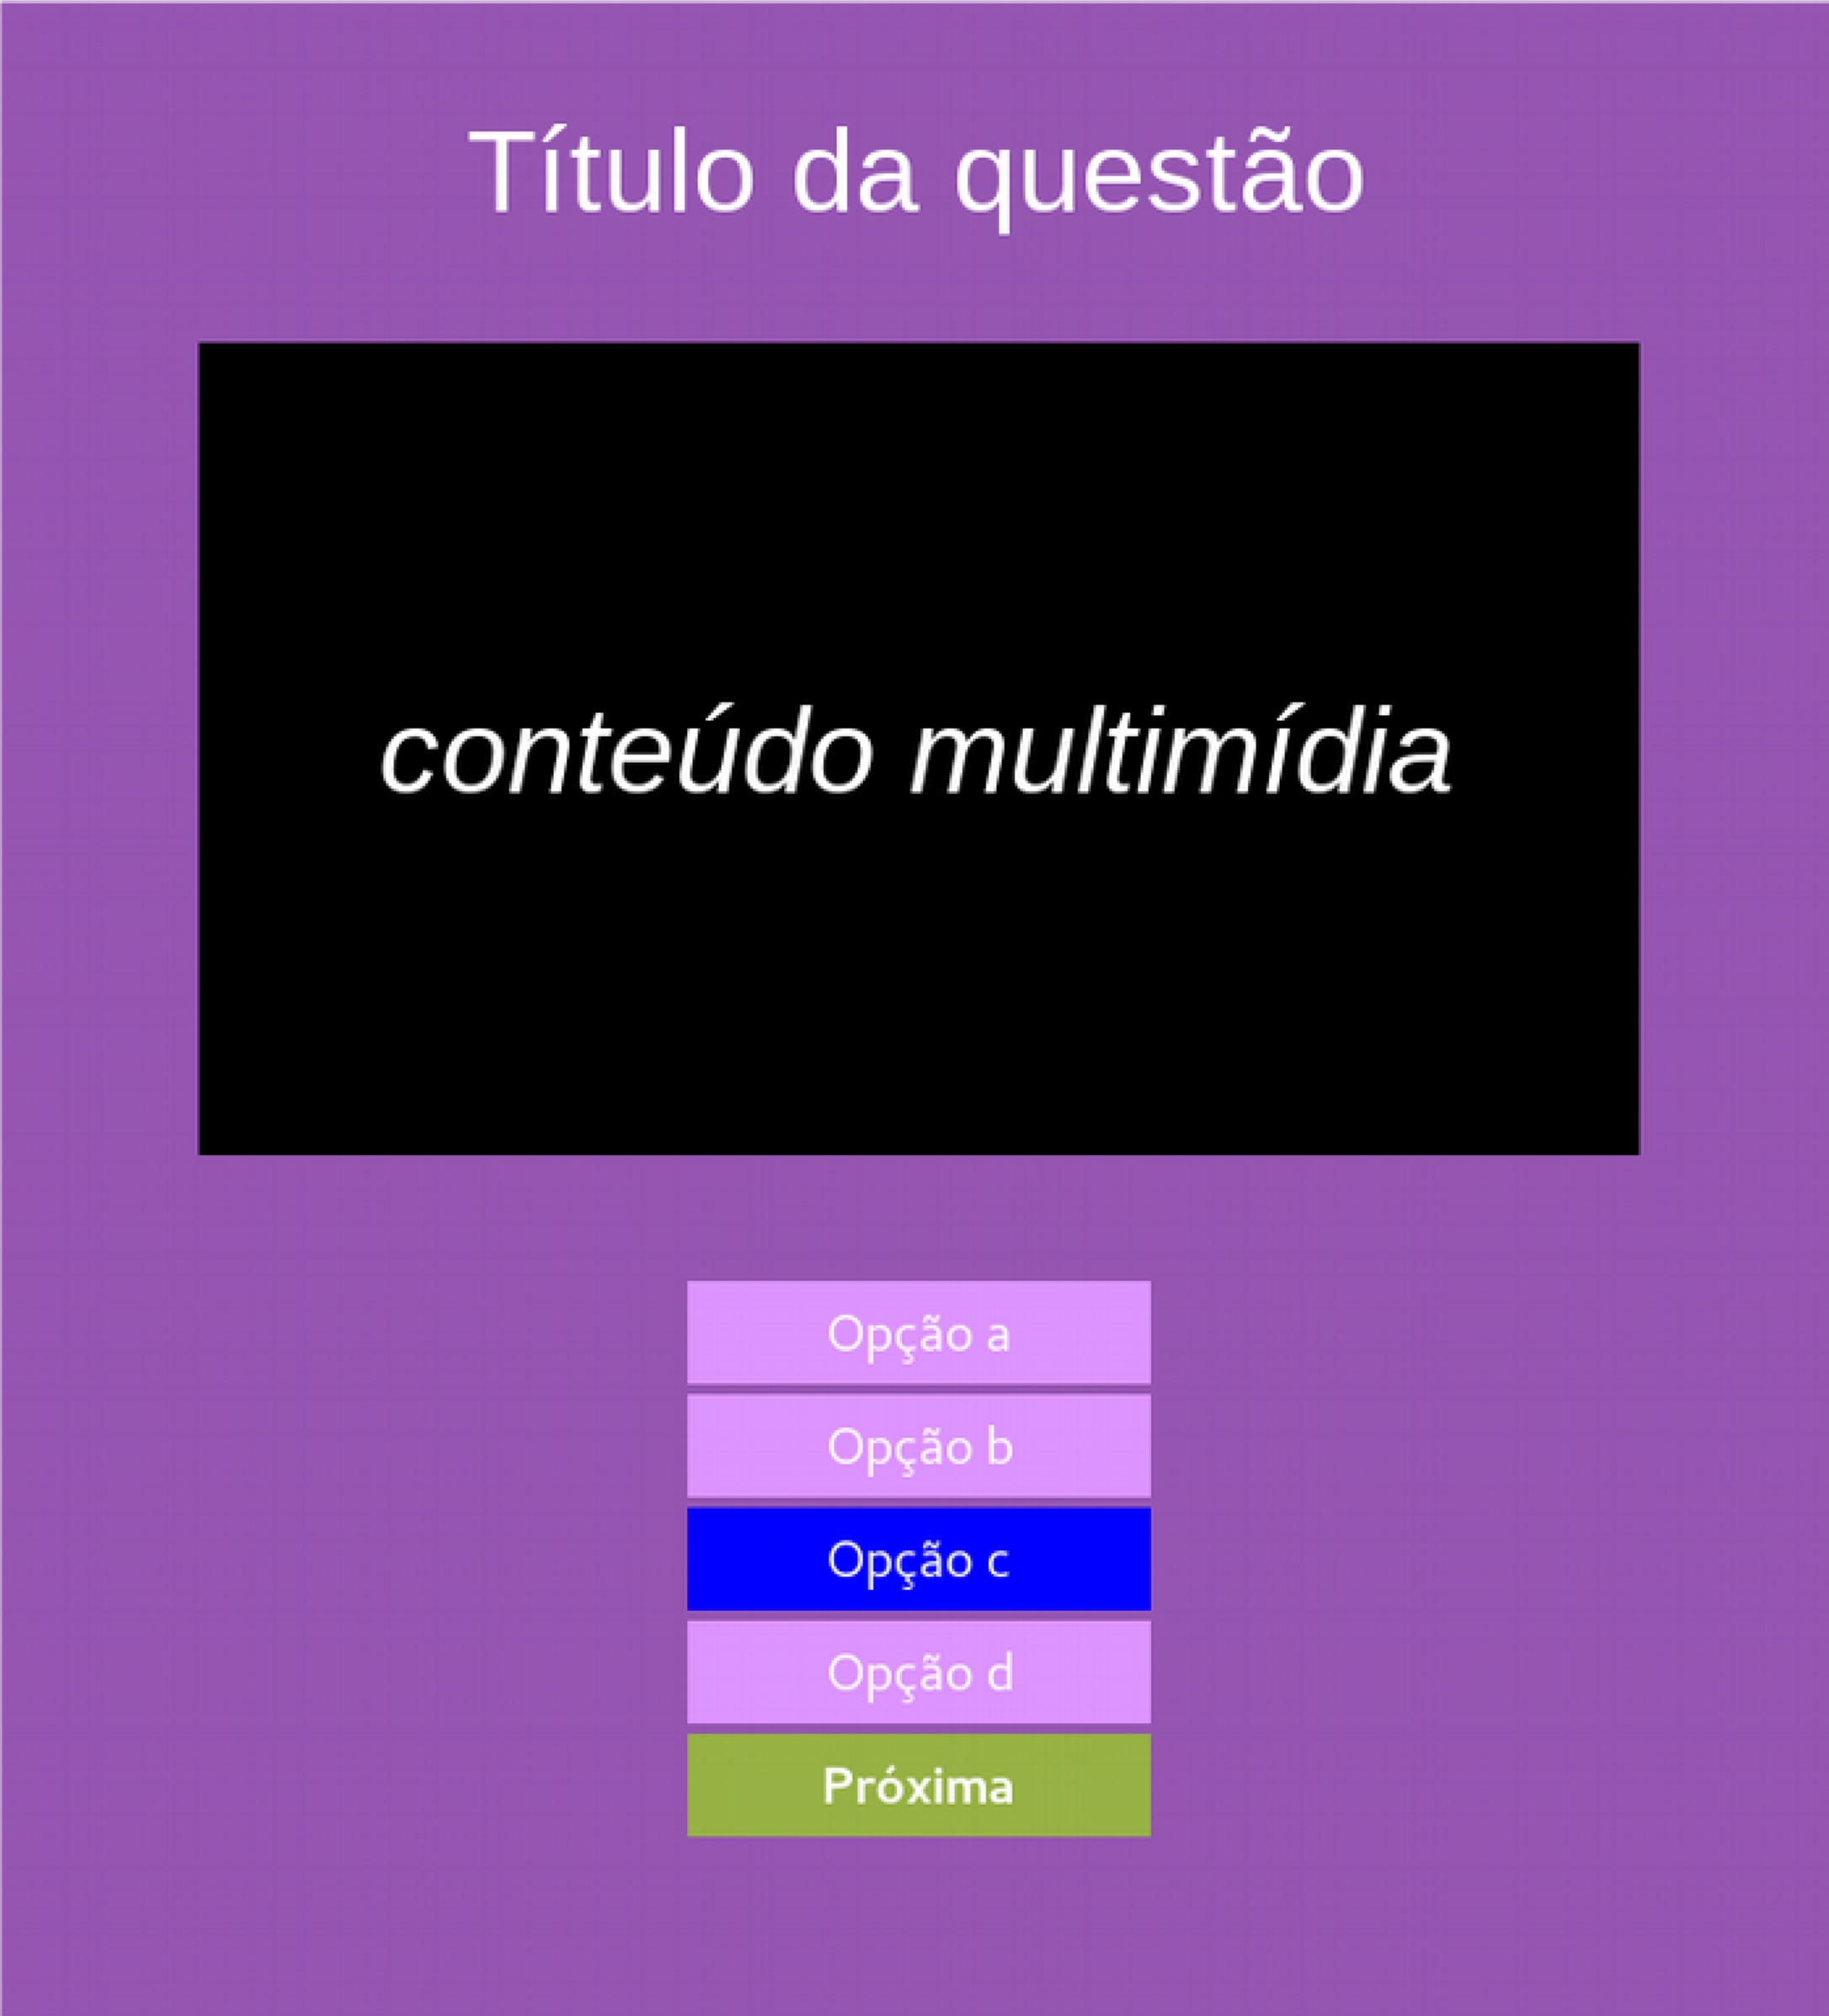
\includegraphics{gui.png}
\end{center}

\begin{center}
\textbf{Figura 1.} \textit{Amostra da interface gráfica do sistema}
\end{center}


\subsection{Referências}
\begin{enumerate}
\item Brusilovsky, P. \& Peylo, C. Adaptive and Intelligent Web-Based Educational
Systems. International Journal of Artificial Intelligence in Education; 2003.
13:156-169.
\item Hobbs, R. Non-optimal uses of video in the classroom. Learning, Media and
Technology; 2006 31, pp. 35-50.
\item Zahn, C., Krauskopf, K., Hesse, F.W., \& Pea, R. Digital video tools in the
classroom: Empirical studies on constructivist learning with audio-visual
media in the domain of history. In: International Conference of the Learning
Sciences. Chicago, IL; 2010.
\item Akhras, F. N. \& Self, J. A. System Intelligence in Constructivist Learning.
International Journal of Artificial Intelligence in Education; 2000 11(4):344-
376.
\item \url{https://www.w3schools.com/tags/tag_video.asp}
\item \url{https://www.w3schools.com/cssref/css3_browsersupport.asp}
\item \url{http://jscc.info/}
\end{enumerate}

\newpage
\section{Arquitetura do sistema}

O sistema é divido em dois módulos: controle e exibição. A parte de controle é responsável por exibir as perguntas salvas no banco de dados na ordem correta de acordo com o que foi planejado pelo instrutor do ambiente de aprendizado e de como o que o estudante está respondendo as perguntas. Já a parte da exibição é responsável por exibir para o aluno as perguntas corretas, juntamente com as mídias relacionadas aquela pergunta. Basicamente, o módulo de exibição é responsável pela interface gráfica do sistema. No começo, o estado do sistema corresponde a caixa \textit{Pegar pergunta do banco de dados} da figura 2, onde ele vai obter a primeira pergunta. O sistema para quando \textit{Verificar se é a última pergunta} for verdade.
\newline

\begin{center}
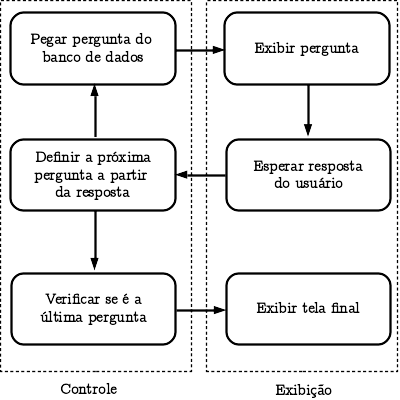
\includegraphics{fluxo}
\end{center}
\begin{center}
\textbf{Figura 2.} \textit{Fluxograma de interação entre os módulos do sistema}
\end{center}

O módulo de \textbf{controle} corresponde ao arquivo:
\begin{itemize}
\item \texttt{js/quiz\_engine.js}: programa que realiza as ações de controle.\\
\end{itemize}



O banco de dados que alimento o \textbf{controle}:
\begin{itemize}
\item \texttt{js/database.js}: base de dados de perguntas que alimentam o \texttt{quiz\_engine};
\item e aos arquivos dispostos em \texttt{/media}, onde ficam as mídias das perguntas.\\
\end{itemize}

O módulo de \textbf{exibição} corresponde aos arquivos:
\begin{itemize}
\item \texttt{html/index.html}: estrutura da tela de perguntas do sistema;
\item \texttt{html/end.html}: tela final do sistema;
\item \texttt{css/style.css}: regras de estilo para os arquivos HTML.\\
\end{itemize}

\section{Código fonte}

Todo o código fonte se encontra em \texttt{src/}

\subsection{\texttt{js/}}
Em \texttt{js/} ficam os arquivos JavaScript, responsáveis pela parte lógica do sistema.

\subsubsection{\texttt{database.js}}

Aqui ficam registrados as perguntas e suas respectivas respostas do sistema. Esse é um arquivo de modelo e seu banco de dados pode ter outros nomes, mas é importante atualizar o nome no resto do sistema. Por padrão, o nome do arquivo é \texttt{database} e o nome da variável do banco é \texttt{db}. O banco é um grande array JSON chamado \texttt{questions}, onde cada elemento é uma pergunta com os seguintes atributos:

\begin{itemize}
\item \texttt{id}: o identificador único daquela pergunta, um número inteiro maior igual que 0.

\item \texttt{title}: o título da questão.

\item \texttt{text}: o texto da questão, a pergunta em si.

\item \texttt{media}: se a pergunta conter algum arquivo de mídia associado, é necessário especificar:

	\begin{itemize}
	\item \texttt{type}: o tipo de arquivo (text, image, audio ou video).
		
	\item \texttt{file}: o arquivo da mídia, dentro da pasta \texttt{media}.
	\end{itemize}

se não houver mídia, o valor deve ser \texttt{null}

\item \texttt{answers}: vetor de respostas de uma determinada pergunta. Cada resposta é composta por:

	\begin{itemize}
	\item \texttt{t}: texto da resposta.
	
	\item \texttt{p}: próxima pergunta que deve ser chamada caso o usuário opte por essa alternativa. Caso não exista próxima pergunta e o programa deve ir para a tela final, colocar o valor -1.
		
	\end{itemize}
	
\end{itemize}

\subsubsection{\texttt{quiz\_engine.js}}

O motor do sistema é o arquivo \texttt{js/quiz\_engine.js}. É ele quem faz a correspondência entre a resposta do aluno e a próxima pergunta. As variáveis globais do programa são:

\begin{itemize}

\item \texttt{var database}: quando atribuída ao banco em \texttt{loadDatabase(name)} é o objeto onde é feita as buscas no banco de dados. Você pode acessar as perguntas usando \texttt{database.question[\textit{n}]}, onde \textit{n} é o número a questão que você quer acessar. De forma análoga, você consegue pegar as respostas \texttt{database.question[\textit{n}].answers[\textit{m}]} e seus respectivos atributos.

\item \texttt{var clickedAnswer = 0}: é a variável que guarda a resposta que o usuário escolheu na pergunta atual, variando de 0 até o \textit{n} - 1, onde \textit{n} é o número de respostas disponíveis (no padrão, 4).

\item \texttt{var actualQuestion = 0}: é a variável que guarda a pergunta atual, começando na primeira pergunta (pergunta número 0).

\item \texttt{var questionsPath = []}: é o caminho que o usuário está seguindo, guardando os \textit{id}s das perguntas por quais ele vai passando.

\end{itemize}

Quanto as funções, elas são:

\begin{itemize}

\item \texttt{function loadDatabase(name)}: carrega o banco de dados de nome \texttt{name} que está no arquivo \texttt{database.js} e coloca na variável global \texttt{database}. O banco é um objeto JSON.

\item \texttt{function begin()}: é a primeira função a ser chamada para iniciar o funcionamento do sistema. Inicia o banco de dados e prepara a primeira pergunta (pergunta 0).

\item \texttt{function setQuestion(num)}: verifica se o quiz acabou (pergunta -1). Se acabou, se direciona para a tela final e passa na URL o \texttt{questionsPath}. Se não é a última questão, vai no banco e busca o texto, a mídia e as alternativas. Coloca o texto no componente HTML adequado. Se a midia existir chama a função \texttt{setMedia(type, file)}, e, senão exitir, só remove a anterior. Pega as alternativas e escreve os textos delas no componente de respostas do HTML.

\item \texttt{function selectAnswer(num)}: pega a resposta escolhida pelo usuário, coloca em \texttt{clickedAnswer} e muda o estilo dos botões, dando destaque para a resposta escolhida.

\item \texttt{function getNextQuestion(answer)}: quando o usuário confirma sua escolha, essa função pega a próxima questão conforme a alternativa escolhida.

\item \texttt{function insertMedia(html)}: insere o trecho HTML passado por parâmetro contendo a mídia na \texttt{div} HTML que comporta as mídias.

\item \texttt{function setMedia(type, file)}: a partir do tipo e do arquivo de mídia passados por parâmetro, gera um código HTML para ser inserido na página.

\item \texttt{function printEnd()}: a partir da URL, pega o caminho das respostas do usuário e coloca no HTML para ser exibido na tela.

\item \texttt{function getUrlVars()}: função auxiliar de \texttt{printEnd()}, que pega os dados da URL.

\end{itemize}

\subsection{\texttt{html/}}
Nesta pasta se encontram os arquivos HTML responsáveis pela estrutura visual da página web.

\subsubsection{\texttt{index.html}}

\begin{itemize}
\item \texttt{head}: metadados da página, como localização dos arquivos JavaScript e CSS e o \texttt{charset}, definido como \textit{UTF-8} possibilita a utilização de caracteres do alfabeto latino (acentos e cedilha). Caso o nome de alguns dos arquivos de \texttt{js/} e \texttt{css/} forem alterados, devem ser alterados aqui também para permitir que a página encontre os arquivos.

\item\texttt{body}: aqui se encontram as estruturas da página. O atributo \texttt{onload}, com o valor \texttt{begin()} significa que essa função será chamada quando a página estiver carregando, fazendo com que a primeira pergunta seja carregada.
\begin{itemize}

\item \texttt{<h3 id="question\_text" \textgreater}: aqui fica o texto da pergunta;

\item \texttt{<div id="media\_div"\textgreater}: divisão para o elemento multimídia;

\item \texttt{<table class="answer\_list"\textgreater}: tabela com as alternativas de respostas possíveis, onde cada célula é um botão. 

\begin{itemize}

\item \texttt{<button class="answer\_button" ...}: Note que cada botão deve ter um \textit{id} único, começando no 0 e indo de forma crescente, da mesma forma que seu parâmetro em \texttt{onclick="selectAnswer(}\textit{id}\texttt{)"} deve ter o mesmo número.

\item \texttt{<button class="control\_button" ...}: Quando este botão é clicado, ele chama a função definida em \texttt{onclick} que, a partir da alternativa selecionada, busca qual a proxima pergunta e prepara a tela com ela.

\end{itemize}

\end{itemize}

\end{itemize}

\subsubsection{\texttt{end.html}}
Esta página exibe a sequência utilizada pelo usuário no sistema, no elemento \texttt{<p id='end'\textgreater}.

\subsection{\texttt{css/}}
Nesta pasta fica o arquivo CSS, responsáveis pelas regras de estilo do HTML.

\subsubsection{\texttt{style.css}}
Esse arquivo define como será a aparência da página, em termos de cor, tamanhos e espaçamentos.

\begin{itemize}

\item \texttt{body}: define a fonte, cor de fundo, cor da fonte, margem e alinhamento do texto.

\item \texttt{.control\_button}: definem as características do botão de confirmação de resposta. Define cor de fundo, cor do texto, tamanho da fonte e tamanho do botão.

\item \texttt{.control\_button:hover}: definem as características deste botão quando o mouse está sobre ele, tornando-o com fundo preto.

\item \texttt{.answer\_button}: definem as características do botão de alternativa de resposta. Define cor de fundo, cor do texto, tamanho da fonte e tamanho do botão.

\item \texttt{.answer\_button:hover}: definem as características deste botão quando o mouse está sobre ele, tornando-o com fundo preto.

\item \texttt{.answer\_button\_clicked}: muda a cor do botão de resposta quando este foi clicado.

\item \texttt{.answer\_list}: retira as margens da lista de alternativas.

\item \texttt{\#question\_text}: define o tamanho do texto da pergunta.

\item \texttt{\#media\_div}: define uma margem para a divisão de mídia.

\item \texttt{.text-body}: remove a margem para o corpo da mídia, quando esta for um texto.

\item \texttt{.text}: define o tamanho da fonte e o alinhamento da mídia, quando esta for um texto.

\end{itemize}

\subsection{\texttt{media/}}
	Nesta pasta devem ser salvas as mídias que serão utilizadas pelo quiz. É importante verificar quais tipos de arquivo são compatíveis com o navegador.
\end{document}

\section{Reconhecimentos}
Esse projeto foi financiado pelo CNPq.